% BAB II Tinjauan Pustaka. Sub-bab baku: Pedoman Tabel 52; isi: Subbab 10.4.
\chapter{Tinjauan Pustaka}
\label{bab:tinjauan}

\panduan{BAB II adalah sintesis yang mengarah ke satu kesimpulan, yaitu
kesenjangan yang akan diisi penelitian, bukan sekadar kumpulan ringkasan artikel
(Subbab 10.4).
Ketentuan rujukan Program Studi Sistem Informasi UNDA:
(1) Total referensi skripsi minimal 30 buah rujukan ilmiah;
(2) Sumber rujukan artikel jurnal nasional wajib minimal terakreditasi SINTA 3 (SINTA 1, SINTA 2, atau SINTA 3) atau jurnal internasional bereputasi (Scopus/WoS);
(3) Rujukan wajib mutakhir (terbitan 5 tahun terakhir, yaitu 2021--2026), kecuali karya klasik/seminal yang menjadi landasan teoritis utama.
Rubrik Sub-CPMK2-CPMK1 memberi nilai tertinggi bila matriks sintesis memuat sedikitnya lima belas artikel jurnal bereputasi lima tahun terakhir (Buku Panduan Dosen, Rubrik CPMK1).}

\section{Landasan Teori}
\label{sec:landasan-teori}

\panduan{Muat hanya konsep yang dipakai langsung pada penelitian dan
hubungkan setiap teori dengan variabel, metrik, atau komponen artefak
yang diukur (Subbab 10.4.2). Jangan mengulang isi buku teks dan jangan
menumpuk definisi kamus.}

Contoh penulisan teori yang langsung terkait metrik: System Usability
Scale (SUS) adalah kuesioner sepuluh butir dengan skala lima poin yang
menghasilkan satu skor kegunaan pada rentang 0 sampai 100
\cite{brooke1996sus}. Cara menghitung skor tersebut dirumuskan pada
Persamaan~\eqref{eq:sus}.

\section{Penelitian Terdahulu dan Matriks Sintesis}
\label{sec:penelitian-terdahulu}

\panduan{Laporkan ringkas protokol tinjauan: pertanyaan riset, basis data,
string pencarian, kriteria inklusi dan eksklusi, jumlah makalah per fase
seleksi PRISMA, dan alat penilaian kualitas. Log pencarian lengkap dan
diagram alir PRISMA ditempatkan di lampiran (Subbab 10.4.1). Ubah matriks
sintesis menjadi narasi tematik yang dikelompokkan menurut tema, bukan
menurut penulis. Setiap tabel dirujuk di teks sebelum tabel itu muncul
(Subbab 11.8).}

Contoh sitasi rentang: tinjauan pustaka yang dapat diaudit memerlukan
pedoman pelaporan, instrumen yang terdokumentasi, dan prosedur
penelusuran rujukan yang dapat diulang
\cite{page2021prisma,brooke1996sus,wohlin2014snowballing}.
Ringkasan sumber yang dipakai disajikan pada Tabel~\ref{tab:matriks-sintesis}.

\begin{table}[htbp]
  \centering
  \caption{Contoh format matriks sintesis penelitian terdahulu}
  \label{tab:matriks-sintesis}
  \begin{tabularx}{\textwidth}{@{}l>{\raggedright\arraybackslash}X>{\raggedright\arraybackslash}X@{}}
    \toprule
    Rujukan & Fokus & Pemakaian pada penelitian \\
    \midrule
    \cite{hevner2004design}      & Pedoman design science research di bidang sistem informasi & Kerangka evaluasi artefak \\
    \cite{page2021prisma}        & Daftar periksa pelaporan tinjauan sistematis & Pelaporan proses seleksi sumber \\
    \cite{wohlin2014snowballing} & Prosedur snowballing untuk studi literatur & Penelusuran rujukan lanjutan \\
    \cite{brooke1996sus}         & Kuesioner kegunaan sepuluh butir & Instrumen pengukuran \\
    \cite{refriansyah2025evaluasi} & Evaluasi usability aplikasi sistem informasi berbasis SUS & Komparasi metrik kegunaan layanan publik \\
    \cite{lupitadyayu2023evaluasi} & Evaluasi usability aplikasi mobile publik skala nasional & Analisis kepuasan dan adopsi pengguna \\
    \cite{eldo2026evaluasi}      & Pengujian usability sistem informasi akademik mobile & Penilaian tingkat akseptabilitas sistem \\
    \cite{zainurrohmah2022evaluasi} & Evaluasi usability website pelayanan perizinan & Validasi instrumen dan kategorisasi SUS \\
    \bottomrule
  \end{tabularx}
  \sumber{olahan penulis}
\end{table}

\section{Kerangka Pemikiran}
\label{sec:kerangka-pemikiran}

\panduan{Kerangka pemikiran memetakan hubungan masalah, teori, metode,
dan luaran, disajikan sebagai gambar bernomor dan dijelaskan di teks
(Subbab 10.4.2). Pada PL1 berupa alur data, praproses, model, dan metrik.
Pada PL2 berupa kebutuhan pengguna, prinsip desain, prototipe, dan ukuran
kegunaan. Pada PL3 berupa kerangka tata kelola atau proses bisnis,
intervensi sistem, dan indikator kematangan atau penerimaan. Gambar
vektor lebih disukai, dan pembeda tidak bergantung pada warna semata
(Subbab 11.8).}

Gambar~\ref{fig:kerangka-pemikiran} memperlihatkan contoh kerangka
pemikiran yang digambar langsung dengan TikZ sehingga tetap tajam saat
dicetak.

\begin{figure}[htbp]
  \centering
  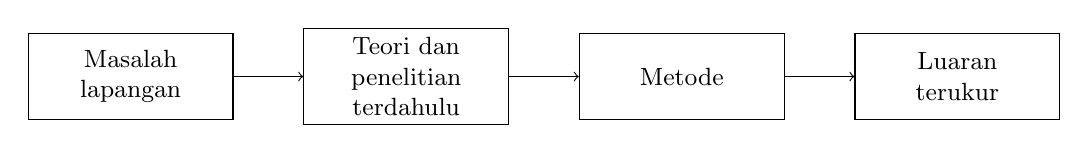
\begin{tikzpicture}[
      kotak/.style={draw,rectangle,align=center,minimum width=2.6cm,
        minimum height=1.1cm,font=\small}]
    \node[kotak] (m) at (0,0) {Masalah\\lapangan};
    \node[kotak] (t) at (3.5,0) {Teori dan\\penelitian\\terdahulu};
    \node[kotak] (d) at (7,0) {Metode};
    \node[kotak] (l) at (10.5,0) {Luaran\\terukur};
    \draw[->] (m) -- (t);
    \draw[->] (t) -- (d);
    \draw[->] (d) -- (l);
  \end{tikzpicture}
  \caption{Contoh kerangka pemikiran}
  \label{fig:kerangka-pemikiran}
  \sumber{olahan penulis}
\end{figure}

\section{Hipotesis}
\label{sec:hipotesis}

\panduan{Subbab ini hanya ditulis bila desain penelitian menguji hipotesis
(Tabel 52). Bila tidak ada, hapus subbab ini.}

Tuliskan hipotesis nol dan hipotesis alternatif beserta uji statistik
yang dipakai untuk mengujinya.
